\chapter{Literature Review}
\section{Unsupervised Learning (SL)}
This is a machine learning task of inferring a function to describe hidden structure from unlabelled data. This type of ML does not require any prior manual categorization of observations in the data. 

The distinction between supervised learning and unsupervised learning (UL) is that in unsupervised learning there is no evaluation of accuracy of the algorithm used, because data fed to the learner is unlabelled . Also one advantage of UL over SL is that time and cost is saved in labelling as required in SL. 
\section{Natural Language Processing (NLP)}
It is a multidisciplinary area that deals with the automatic processing of human language. 
This automation allows communication between humans and computers. The computer accept input in the form of text or speech and then produces structured representations showing the meaning of those strings as their output.


%\Jnote{Explain what is appeal and what is appeal id.}

\section{Word Embeddings}
Word embeddings is a dense representation of words in a low dimensional vector space. Bigo et al(2003) introduced the  concept of word embedding and then train them in neural language jointly with model parameters. \citep{mikolov2013distributed} came out with the popular word embedding model known as the Word2vec. 
\cite{faruqui2014retrofitting} released Glove. The Glove and the Wor2vec are both aimed at producing word embeddings that ecode the general semantic relationship.
\section{Topic Model}  
A topic model is a statistical tool that produce a short description of an original document. Topic models can be applied on a single document or a collection of documents. \citep{blei2012surveying} described topic models as algorithms that discovers the main themes existing in a large text or document and otherwise the combination of two or more documents. He further reveal that the development of probabilistic topic modelling by ML  researchers as a set of algorithms that is geared towards revealing and describing large archives of documents with thematic information. Topic models analyses words in the large text document to discover the themes that pervades them, the connection that exist between the words and their occurrence with time. In topic modelling the stress of having to label the documents prior to annotations is saved as it is been done in supervised learning. from the analysis of the original document the topics are obtained. Given a very large volume of electronic archives that is impossible for human annotations, topic modelling can help to summarize and organize it.
\section{Topic Model methods}
Topic modelling techniques have been developed to automatically summarize document or large text. These techniques are: latent semantic indexing/allocation  (LSI/LSA), the latent dirichlet allocation (LDA) and the probabilistic latent semantic analysis (PLSA) . This research will be restricted to LDA and LSA.
%\Jnote{s/narrow between/be restricted to} 
\section{Vector Space Model (VSM)}
%\Jnote{I thought what you describe here is called ``bag of words''. Can
 % you explain the difference?}

In Natural Language Processing (NLP) specially in semantics similarity documents can be represented as a vector of words in in a vector space model \cite{salton1975vector}. The frequency of the word in the document determines its importance. Given two documents with words  "desk" and "shirt". From the matrix table below "desk" appears 6 and 4 times in document 1 and document 2 respectively, and the word "shirt" appears 3 times in document 1 and 5 times in document 2. Geometrically this can be represented as shown in \eqref{figure 2.1}.
%\Jnote{Put quotes around ``desk'' and ``shirt''.}
\captionof{table}{ Document of words}
$$\begin{array}{cccc}
 &\text{desk} & \text{shirt} \\ 
 Doc_1 & 6 & 3\\ 
 Doc_2 & 4 & 5
\end{array} $$

\begin{figure}[hbtp]
\centering
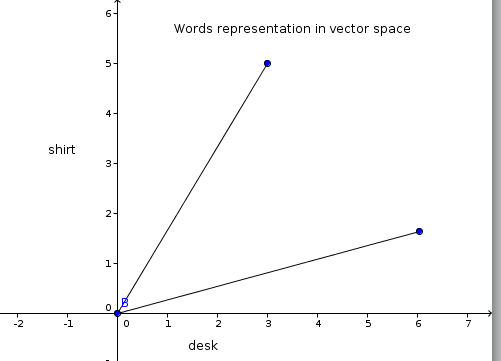
\includegraphics[scale=1]{words_in_vs.png}
\caption{Words represented in vector space}
\end{figure}
\label{figure 2.1}
Computing the distance between them tells the extent to which their similarity. The dot product shows how close the two vectors are to each other. The dot product of two vectors is given as
$$X\cdot Y=|X||Y|\cos (\theta) \text{.}$$
%\Jnote{Use straight font for functions like cos. This can be achieved
%  by writing ``\textbackslash cos'' instead of ``cos''.}
%\Jnote{Dot should be inside the equation, not after on the next line.
%  Typically I write something like
%as ``\textbackslash cos(\textbackslash theta) \textbackslash; .''}

Although the VSM is a simple model to use, one main limitation is that, it cannot handle polysemy and synonyms issues. Polysemy is a term that describes words with multiple meaning and synonyms are words that have similar meaning.
For example, a polysemy word such as "light" can be used in the context of weight of an object or to describe a type od electromagnetic radiation.
Words like "detect", "find", "uncover" and "reveal" are synonymous, they can be used to describe a particular event.

%\Jnote{Give clearer explanations of what is polysemy and what are synonyms.
%  Consider giving an example.}
Considering a query search in Google, by the SVM, the documents relating to the query will not be revealed in the search results. However a research conducted by Erk and Pado pointed out the reason leading to the limitations in SVM.
%\Jnote{Reason behind the reason?}
The paper indicated that the existing model does not take syntatic structure into account. Their research resulted in a model called "structured vector space (SVS)". This work incorporates the context in which words are used.
%\Jnote{Novel is a type of book, you mean something else.} . selectional preferences for words argument position. With this it is possible to integrate syntax computation of word meaning in context. \Jnote{I don't understand at all,
%  please explain better.}
%
%\Jnote{You have to use more paragraphs and less sections. Sections should be,
%  e.g., VSM, LSA and LDA, not so many as now. On the other hand, you should
%have many more paragraphs. General rule: One thought, one paragraph.}

\section{Latent Semantic Analysis (LSA)}
\begin{flushleft}
Also known as the latent semantic indexing (LSI) is a topic model method
that transforms documents of high dimension to low dimension of words. One useful role played by LSI in topic modelling is its ability to deal with polysemy and synonyms \cite{deerwester1990indexing}.
\end{flushleft} 
Preliminarily it constructs a matrix $M\in \mathbb{R}^{n*k}$, from the documents $d_1, d_2,..., d_k$ of words $w_1, w_2, ... w_n$. The rows represents the different words and the columns can be viewed as different documents.
%\Jnote{Are you sure? It feels to me you switched rows and columns.}
For example from \eqref{Table 2.1}, $m_{ij}$ shows the position and the frequency of the word $w_i$ in document $d_j$.
To achieve reduction in the dimension of the matrix $M$ the truncated Singular Value Decomposition is applied, given as:
$$M\approx A_t \sum B^{T}_t.$$
$A_t$ and $B^T$ are orthogonal matrices, whilst $ \sum$ is a diagonal matrix.
Reducing the dimension leads to reduction of noise \cite{deerwester1990indexing}.
%To find similarity of words, compute the cosine values of their vectors. \Jnote{I don't understand last sentence, please explain better.}
\captionof{table}{Corpus of documents}
$$\begin{array}{cccc}
 &d_1 & d_2 &d_3 \\ 
 \text{food} & 0 & 0 & 2 \\ 
 \text{school} & 2 & 5 & 0 \\ 
 \text{cash} & 0 & 1 & 0 \\ 
 \text{automobile} & 1 & 0 & 4
  \end{array} $$
%  \Jnote{What is this table about? Why is ``food'' listed twice? Please explain.}
%$$\text{fig. 1}$$
%\section{Probabilistic Latent Semantic Analysis  (PLSA)}
\section{ Latent Dirithchet Allocation (LDA)}
\begin{flushleft}
Blei(2012) referred to LDA as the simplest topic model . The ideas underlying this model is every document has several topics existing in it.He defined topic to be a distribution over a fixed a vocabulary.
%\Jnote{Topic is a distribution over a topic?}
Each topic is made up of words that are very related to the topic. Considering an article with a title "Seeking Life’s Bare (Genetic) Necessities,” for which data analysis was used to determine the number of genes an organism needs to survive. By hand, words pertaining to three different vocabularies were highlighted with different colours. Words such as "computer", "prediction" linked to the topic "data analysis" highlighted blue, "life" and "evolve" about "evolutionary biology" highlighted pink and words like "gene", "DNA" describing the topic "genetics" is highlighted yellow.
%\Jnote{Put respective words in quotes.}
Stop words that occur frequently in the article are removed. 
\end{flushleft}

The LDA as a statistical tool uses this idea based on the assumption that topics are generated prior to words assignment. The LDA also assumes a model of generating documents. All words in each vocabulary has a probability value and depending on the topic each word finds itself would be high or low. For example the word "gene" will have a low probability value if it is in the domain of the  vocabulary "data analysis" compared to when it belongs to the topic "genetics". 

The idea describing the process of generating documents using words is:
\begin{itemize}
\item[1.] From the documents, a random selection of some topics deemed to describe the documents.
\item[2.] for each word in the documents:
		\item[2a.]Randomly choose a topic from
the selected topics in step 1.
		\item[2b.]Randomly choose a word from the selected topic. The topic ha s a collection of words of which randomly one is chosen at a time. 
\end{itemize}
%\Jnote{I don't understand how the process above works, please explain
%  better.}
The LDA model reflects the idea of multiple topics exhibited by documents.

Figure\eqref{Figure 2.2}  gives a picture of the whole intuition of this generative probabilistic process:

\begin{figure}[hbtp]
\centering
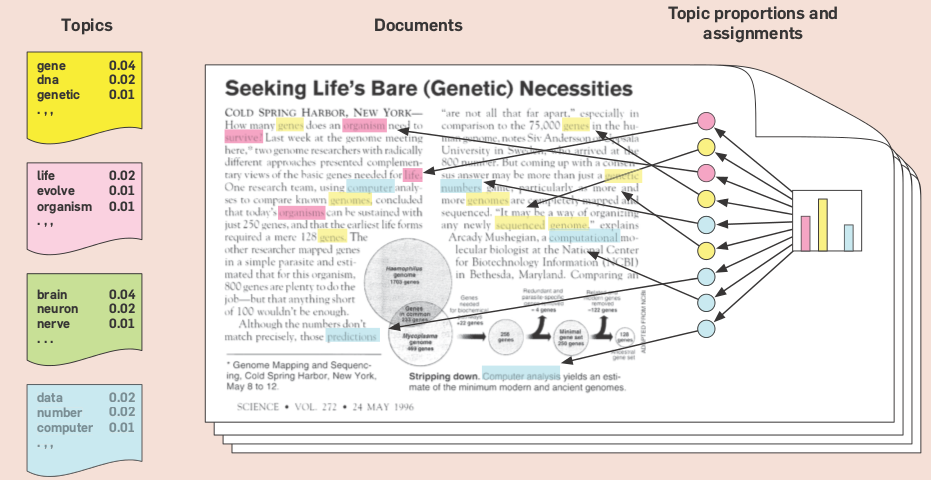
\includegraphics[scale=0.5]{DLA.png}
\caption{Generating documents by reverse process of the LDA model}\label{Figure 2.2}
\end{figure}
In short description of Figure \eqref{Figure 2.2} the idea underlying LDA is that, first of all some number of topics that are distribution over words is assumed (far left). In generating for each document, firstly choose a distribution over topics (far right ie. histogram), then the circles of different colours are topic assignment for which words drawn from the document corresponds to.

Figure \eqref{Figure 2.3} shows real inference with LDA, using 17000 articles from the journal of science. "Genetics", "Evolution", "Disease" and "Computers" represents the topics  from one article and the words below each are top 15 most frequent words. The graph on the left shows the probability values for each topic.
The probability values for this article for a given set of topics may be different from another article. in effect, even though some documents or articles may share the same topics, each article exhibits the topics in different proportions.
\begin{figure}[hbtp]
\centering
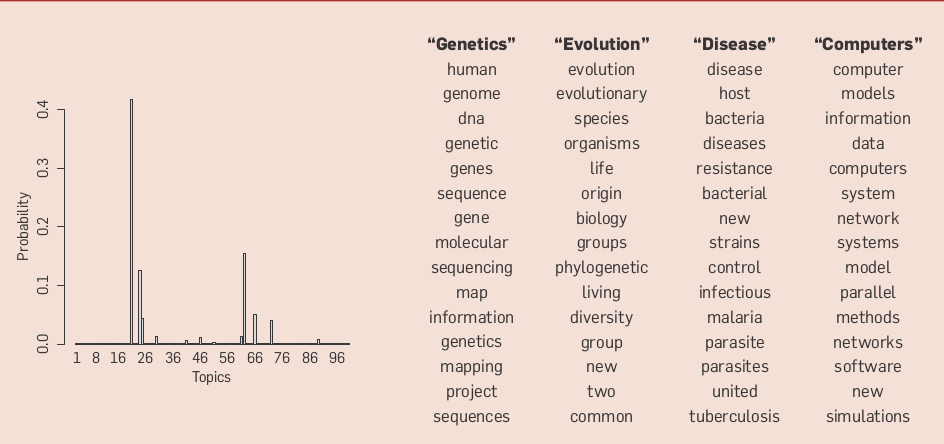
\includegraphics[scale=0.5]{infered_topics.png}
\caption{Infered topics from one article of the 17000 articles froom the journal of science.}
\label{Figure 2.3}
 \end{figure} 
\section{Graphical Model of LDA}
Figure \eqref{Figure 2.3}provides a graphical representation, showing the both the observed and latent variables involved in the generative process. Latent variables are variables that are not directly but inferred from the the observed.
%\Jnote{What is latent variable? Please explain.}
The only observed part is the shaded circle $W_{d,n}$ , $\alpha$ and $\eta$ are parameters from the Diritchlet distribution.
\begin{figure}[hbtp]
\centering
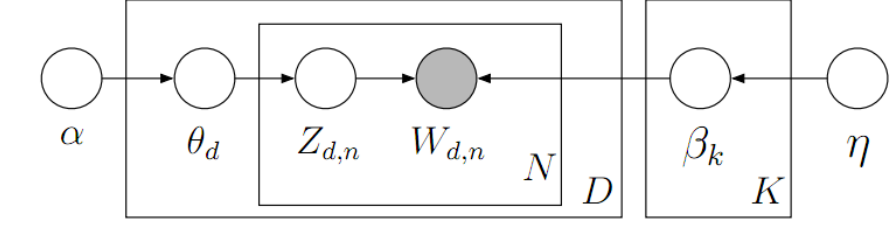
\includegraphics[scale=0.5]{Graphical.png}
\caption{Graphical representation of LDA model} \label{Figure 2.3}
\end{figure}
What the notations stands for:
\begin{itemize}
\item$D$:the number of documents
\item$N$: number of words in each document
\item$K$: number of topics
\item$\theta_d$: the topic proportion for each document $d$.
\item $Z_{d,n}$: is the topic assignment for word $n$ in document $d$.
\item $W_{d,n}$: is the observed worn $n$ in document $d$,
\item $\beta_K$:topics
\end{itemize}
From \eqref{Figure 2.3} the joint  distribution or the total probability of both latent and observed variables is given by:
\begin{align}
P(\beta,\theta,Z,W, \alpha, \beta )=\prod_{k=1}^{K}P(\beta_i)\prod_{d=1}^{D}P(\theta_d)
\prod_{n=1}^{N}P(Z_{d,n}|\theta_d)P(W_{d,n}|\beta_k,Z_{d,n})
\end{align}
\section{Posterior Distribution}
This is a type of Bayesian statistic that describes how  latent variables are obtained given the observed data. From the LDA documents generative model a joint probability distribution of both the hidden structures and observed variables. To compute the conditional distribution given the observed variables (words), the posterior is used, given by:

$$P(\theta_{1:D},\beta_{1:K},Z_{1:D}|W_d)=\frac{P(\theta_d,\beta_k,Z_d,W_{1:D})}{P(W_{1:D})}\text{.}$$
$P(\theta_d,\beta_k,Z_d,W_{1:D})$ can be computed easily for any setting of the hidden variables. $P(W_{1:D})$ is the marginal probability of the observed word variable. This is computed by considering all possible instances of the hidden topic structure by summing the their joint distribution. Because the possible topic structure is large, it is very hard to compute using this posterior relation.

There exist a number of algorithms categorized as "sampling based algorithms" and "variational based algorithms". These algorithms approximate the posterior distribution based on the joint probability distribution between the latent variables and the observed in the posterior relation.

\section{Variational Bayes (VB)}
This is a method for approximating the posterior distribution. Recalling from the difficulty encountered by the posterior in computing the marginal probability of the observed variable $P(W_{1:D})$. This form of approximation operates when we have both observed and hidden variables, but also latent parameters.

The VB serves two purposes, of which are:
\begin{itemize}
\item VB gives an analytical approximation to the posterior probability given the observed and latent variables, so as to use the approximate values to make some inference.
\item To determine from it a lower bound for a marginal probability of the observed data, also known as the evidence. That is, it is the marginal probability of the data given the model. 
This idea is used to select a best model, on the premise that the model with the highest marginal likelihood shows a best of the data by the model. This also justifies that there is a high probability that the used was generated by the model.
\end{itemize}
\section{Diritchlet Distribution}
It is from the exponential family of continuous multivariate probability with the parameter $\alpha$ of positive real. It is denoted by $D(\alpha)$.

Suppose $S=[S_1,S_2,...,S_d] $  represent the  probability mass function (pmf), for each $S_i\geq 0$, then $\sum _{i=1}^{d}S_i=1$. Also suppose $\alpha=[\alpha_1,\alpha_2,...,\alpha_d]$ with $\alpha_i>0$ for each $i$, and let $\alpha_0=\sum _{i=1}^{d}\alpha_i$. Then $S$ is said to have a Dirithchlet distribution with parameter $\alpha$, which is denoted by $S \backsim $Dir($\alpha$), if $s$ is a  pmf then,
\begin{align}
f(s,\alpha)=\frac{\Gamma(\alpha_0)}{\prod_{i=1}^{d}\Gamma(\alpha_i)}\prod_{i=1}^{d}s^{\alpha_i -1}.
\end{align}
However if $s$ is not a pmf  it has $f(s,\alpha)=0\text{.}$

Where $\Gamma()$ is the Gamma distribution.
%\Jnote{Please, I didn't understand a single sentence in this section.}
\section{Advantages of LDA} 
LDA can be used as a built in module in other models to perform more difficult tasks.
The LDA model is used in other applications, not only in text.(Blei and Jordan,2002) carried out a  work that used pairs of LDA modules to
model relationships between images and their corresponding descriptive captions .
%\Jnote{Who is ``we''? Please don't copy sentences from papers.}
But also include problems involving collections of data, including data from domains such as collaborative filtering,
content-based image retrieval and bioinformatics.
\section{Disadvantages of LDA}
The bag of words assumption (the order words in a document does not matter) of LDA makes it unrealistic, however it is reasonable if only our task is to uncover the course thematic structure of the texts (Blei,2012).
\section{Extentions of LDA}
\cite{wallach2006topic} developed a model that does not ignores the assumption that the order of words does not matter (bag of words). This means that the each word generated by the topic depends on the previous word. 
%uses the combination of the n gram statistic and latent topic variable by extension of the uni-gram topic model to include properties of a hierarchical Dirichlet language model. n gram statistics is a close collection of sequence of items from a text or speech. Uni-gram is at type of  n gram model of size one.
%\Jnote{Please don't copy sentences from papers. I hope you can explain to me:
%  What is n-gram statistic? What is latent topic variable? What is uni-gram topic model? What is a hierarchical Dirichlet model?}
\cite{griffiths2007topics} combined the idea of syntactic and semantics to produce a generative model. This model  is capable of simultaneously finding syntactic classes and semantic topics despite having no knowledge of syntax or semantics beyond statistical dependency
%Text text text text text text text text text text text text text text
%text text text text text text text text text text text text text text.
%
%When you get stuck, don't panic. 
%The world is unlikely to end just now. 
%Remember you can consult your supervisor, tutor, and Blaise at agreed times. 
%
%\begin{thm}[Jeff's Washing Theorem]
%\label{thm:jwt}
%If an item of clothing is too big, then washing it makes it bigger;
%but if it is too small, washing it makes it smaller.
%\end{thm}
%\begin{proof}
%Stated without proof. But a proof would look like this. 
%\end{proof}
%
%Notice that no Lemmas are required in the proof of Theorem \ref{thm:jwt}.
